\section{Einphasen-Stromrichteröltrafo 16.7 Hz}
Der \SI[]{16.7}[]{\Hz} Transformator ist ein Summiertransformator und addiert die
Teilspannungen der Umrichterr auf die Bahnspannung 2 AC
\SI[]{110}[]{\kV}. Der Transformator ist ölgefüllt, selbstkühlend und für die Aussenaufstellung ausgelegt.

\subsection{Allgemeine Merkmale}

\begin{table}[htb]
    \centering
    \begin{NiceTabular}{|l|c|}[]
        \CodeBefore
        \columncolor{lightergray}{1}
        \Body
        \hline
         Aufstellung & Freiluftaufstellung\\
         \hline
         Verschmutzung & Verschmutzungsgrad III (stark) \\
         \hline
         Aufstellungshöhe & < 1000 m üNN\\
         \hline
         Umgebungstemperatur &  -30°C bis 40°C\\
         \hline
         Klimabedingungen & Normal\\ 
         \hline
                 \Block{3-1}{Dokumentationen} &  \tabitem Technische Zeichnungen und CAD\\
                         &\tabitem Montageplan, Wartungsplan, Dokumentationen\\
                         &\tabitem Prüfprotokoll der zu erfüllenden Prüfungen\\
            \hline
    \end{NiceTabular}
\end{table}

\textbf{Normen:}

\textbf{Schaltbild}
\begin{figure}[htb]
\centering
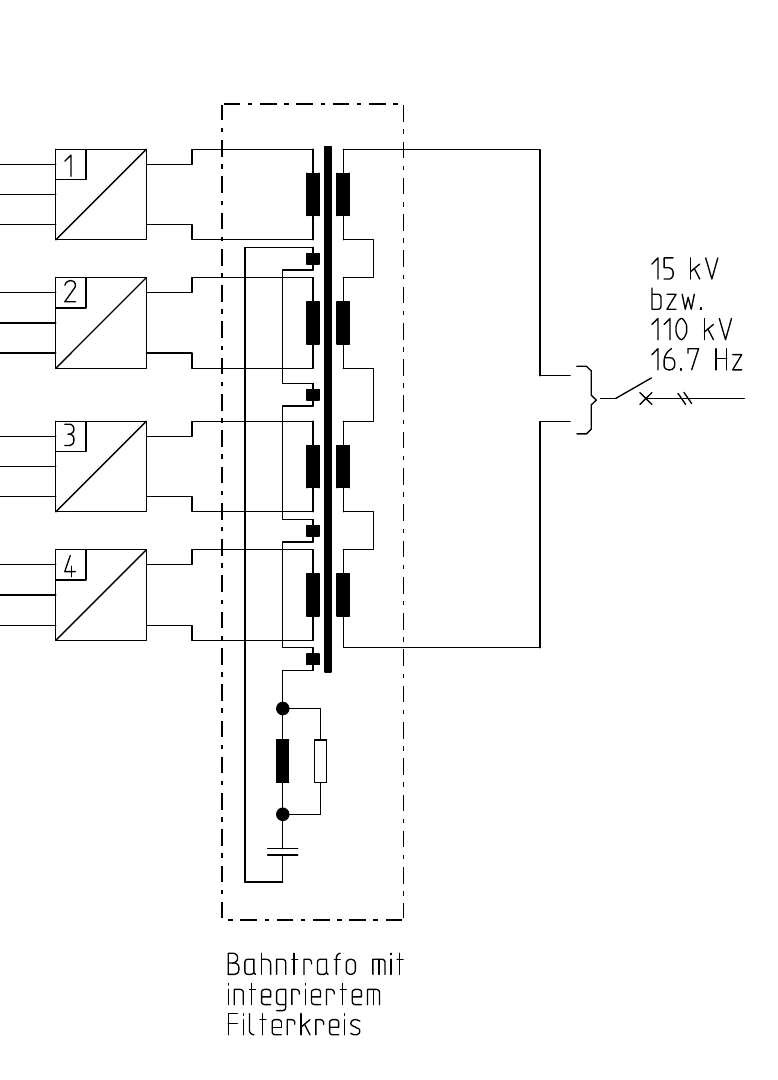
\includegraphics[width=\textwidth/3,frame]{Bilder/stromrichtertrafo.png}
\end{figure}

\textbf{Bemessungsdaten:}
\begin{table}[htb]
    \centering
    \begin{NiceTabular}{|l|p{2cm}|p{2cm}|}[hvlines]
        \CodeBefore
        \columncolor{lightergray}{1}
        \Body
       \Block{2-1}{Schaltgruppe} & OS & US \\ 
                                & | &   i0i0i0  \\
         Nennleistung ohne Leistung der Filterwicklung & \Block{1-2}{$\SI{20}{\unit{\mega\volt\ampere}}$}\\
         Leistung US Wicklung & \Block{1-2}{$4\cdot\SI{5.125}{\mega\VA}$}\\
         Nennfrequenz nach DIN EN 50163/A1 \cite{DeutschesInstitutfurNormungene.V..200802} & \Block{1-2}{$\SI{16.7}{\Hz}-6\%+4\%$}\\
         Nennspannung der OS-Wicklung  & \Block{1-2}{$\SI{110}{\kilo\V}$}\\
         Nennspannung einer US Wicklung bei \SI[]{110}[]{\kV} & \Block{1-2}{$4\cdot\SI{3535}{\kV}$}\\
         Nennstrom US-Wicklung bei Nennspannung & \Block{1-2}{$\SI{1414}{\A}$}\\
        Filterwicklung (HW) Nennleistung & \Block{1-2}{$\SI{4.8}{\mega\VA}$}\\
        Filterwicklung (HW) Nennspannung & \Block{1-2}{$\SI{6}{\kilo\V}$}\\
    \end{NiceTabular}
\end{table}

\textbf{Kurzschlussspannung, Impedanzen}
\begin{table}[htb]
    \centering
    \begin{NiceTabular}{|l|p{2cm}|p{2cm}|}[hvlines]
        \CodeBefore
        \columncolor{lightergray}{1}
        \Body
       \Block{2-1}{Schaltgruppe} & OS & US \\ 
                                & Y(N) &   i0i0i0  \\
         Nennleistung ohne Leistung der Filterwicklung & \Block{1-2}{$\SI{20}{\unit{\mega\volt\ampere}}$}\\
         Leistung US Wicklung & \Block{1-2}{$4\cdot\SI{5.125}{\mega\VA}$}\\
         Nennfrequenz nach DIN EN 50163/A1 \cite{DeutschesInstitutfurNormungene.V..200802} & \Block{1-2}{$\SI{16.7}{\Hz}-6\%+4\%$}\\
         Nennspannung der OS-Wicklung  & \Block{1-2}{$\SI{110}{\kilo\V}$}\\
         Nennspannung einer US Wicklung bei \SI[]{110}[]{\kV} & \Block{1-2}{$4\cdot\SI{3535}{\kV}$}\\
         Nennstrom US-Wicklung bei Nennspannung & \Block{1-2}{$\SI{1414}{\A}$}\\
        Filterwicklung (HW) Nennleistung & \Block{1-2}{$\SI{4.8}{\mega\VA}$}\\
        Filterwicklung (HW) Nennspannung & \Block{1-2}{$\SI{6}{\kilo\V}$}\\
    \end{NiceTabular}
\end{table}
